\documentclass[conference]{IEEEtran}
\IEEEoverridecommandlockouts
% The preceding line is only needed to identify funding in the first footnote. If that is unneeded, please comment it out.
\usepackage{cite}
\usepackage{amsmath,amssymb,amsfonts}
\usepackage{algorithmic}
\usepackage{graphicx}
\usepackage{textcomp}
\usepackage{xcolor}
\graphicspath{{./Screenshots}}

\def\BibTeX{{\rm B\kern-.05em{\sc i\kern-.025em b}\kern-.08em
    T\kern-.1667em\lower.7ex\hbox{E}\kern-.125emX}}
\begin{document}

\title{Optimal Routing using the In-band Network Telemetry Framework with P4 Switches\\}

\author{\IEEEauthorblockN{Shikhar Gupta}
\IEEEauthorblockA{School of Computing \& Augmented Intelligence \\
Arizona State University \\
sgupt330@asu.edu}
\and
\IEEEauthorblockN{Kiran Sthanusubramonian}
\IEEEauthorblockA{School of Computing \& Augmented Intelligence \\
Arizona State University \\
ksthanus@asu.edu}
}
\maketitle

\section{Introduction}
Rapid progress has been made in programmable data planes in the past few years. The P4 programming language \cite{b1} has seen considerable adaptation to make the programmability of switches protocol and hardware independent. It enhances the use of Software Defined Networking and the OpenFlow API to configure forwarding devices and network behavior determination in a “top-down” approach.  With the advent of P4, the overall programmability and ease of reconfigurability of the data plane have significantly increased. The implementation of P4 has also led to a variety of new use cases and research areas, such as DDoS Attack Prevention \cite{b2}, improving Network Resilience paradigms \cite{b3}, Load Balancing \cite{b4}, and Traffic Engineering \cite{b5}.

Within the P4 specification, the In-band Network Telemetry (INT) Framework has emerged to gather real-time information from the data plane. Active and passive network monitoring techniques have been used significantly to monitor network data resource usage. However, active monitoring does not give an accurate report on the network’s performance, whereas passive networking is effective but has a high processing overhead that can lead to performance limitations. The INT Framework provides a means of performing network telemetry calculations within the data plane. There has been significant development in designing efficient monitoring systems through INT, such as IntMon \cite{b6} and INT Collector \cite{b7}.  INT has also seen practical use in cases such as event detection \cite{b8}, queue measurement \cite{b9}, and improved real-time slice monitoring \cite{b10}. It has also made inroads in defining a new blend of Network architectures \cite{b11}.

P4 and INT can also optimize routing strategies between multiple hosts. P4 switches have also been used as a backbone to create software systems for performance-based ISP routing \cite{b12}. P4 and INT have also minimized latency in autonomous networks with AI-based forecasting \cite{b13}.

\section{Problem Statement}
The primary motivation for this problem statement is to gain a deep understanding of P4 Programming, specifically configuring an INT Switch Topology for network monitoring purposes. We will examine the different modes of operation offered while using the INT Framework (Fig. 1). With the telemetry information, we intend to make real-time reconfigurations to the Open Shortest Path First (OSPF) routing protocol in our Controller Node and propagate forwarding table changes to the P4-based Programmable Switches using P4Runtime. The entire topology will be deployed as a slice on the FABRIC Testbed.

The objective is to optimize the dedicated resources and the overall bandwidth, and minimize latency across the entire network slice. The whole slice-level metrics will be measured using the Measurements Framework Library (MFLib) present in the FABRIC Testbed. Using the MFLib API will enable us to have a definitive way to store our metrics in ElasticSearch and easily connect to Grafana for Data Visualization purposes.

\section{Methodology}
In this section, we define the project flow to execute the requirements outlined in Section 2. 

First and foremost, we describe the topology used for our experiments (illustrated in Figure 2). Host 1 acts as the SDN Controller used to run P4Runtime to configure the switches in the topology. It will also determine the routing protocol configuration to make real-time optimizations in the routing strategy used to transfer data to the receiving destination host (i.e., Host 2). The switches defined are completely programmable BmV2 P4 switches. Each switch performs critical tasks to implement the INT Framework. We describe the different INT Switch Roles as follows:
\begin{enumerate}
\item \textbf{INT Source}: Creates and inserts INT Headers into the packets it sends. A Flow Watchlist is configured to select the flows in which INT Headers are to be added/modified.
\item \textbf{INT Sink}: Extracts the INT Headers and collects the path state contained in the INT Headers. The collected information is sent to the monitoring system for further processing and storage.
\item \textbf{INT Transit Hop}: Collects metadata from the data plane by following the INT instructions. 
\end{enumerate}

The information collected in the INT Headers will include metrics such as hop latency and buffer queue time. The Network Monitor stores the information collected from the INT Packets. A critical function of the Network Monitor is efficiently detecting important network events while balancing with minimizing computation overheads and adding latency to the overall network. \\

\begin{figure}[htbp]
\centering
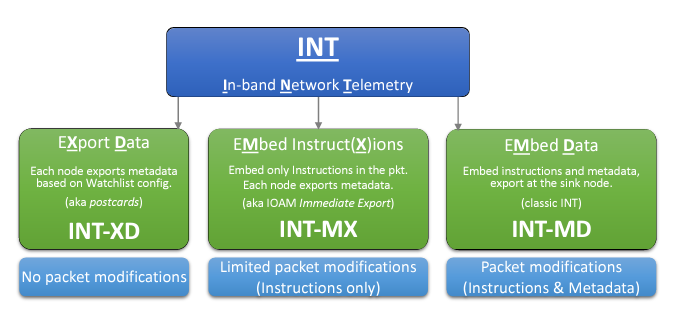
\includegraphics[scale=0.5]{INT_Modes_of_Operation.png}
\caption{INT Modes of Operation \cite{b14}}
\label{fig}
\end{figure}

Secondly, using the information processed and stored using the INT Framework, we wish to dynamically modify the initial routing strategy based on hop latency, traffic flow rate changes, etc. This will also include dynamically reconfiguring the forwarding tables in the P4 switches.

Lastly, we will attempt to demonstrate the effects of the routing modifications on the network slice’s overall throughput and latency compared to the original approach used.

\section{Project Deliverables}
The following are the incremental steps we will follow during the course of the project:
\begin{enumerate}
\item Walkthrough of P4 tutorials; implementing and deploying a basic P4 program on FABRIC.
\item Writing customized P4 programs for implementing the INT Specification. This includes analysis of the three modes of INT operation and setting up a basic topology with INT Sources and Sinks.
\item Setting up the proposed topology on FABRIC, implementing the entire telemetry system with minimal network and processing overheads, and visualizing the telemetry gathered when the hosts communicate. This stage will also include writing a codebase using the MFLib API to monitor and log network slice information continuously.
\item Devising a dynamic optimal routing strategy based on the telemetry gathered.
\item Devising a means of dynamically changing the route forwarding tables based on the new optimal routing strategy and observing the changes.
\item Visualize the telemetry and slice information based on overall throughput and latency. We will also attempt to visualize a simulation showcasing the dynamic route switching capability.
\end{enumerate}

\begin{thebibliography}{00}
\bibitem{b1} Pat Bosshart, Dan Daly, Glen Gibb, Martin Izzard, Nick McKeown, Jennifer Rexford, Cole Schlesinger, Dan Talayco, Amin Vahdat, George Varghese, and David Walker. 2014. “P4: programming protocol-independent packet processors”. SIGCOMM Comput. Commun. Rev. 44, 3 (July 2014), 87–95

\bibitem{b2} Damu Ding, Marco Savi, Domenico Siracusa, “Tracking Normalized Network Traffic Entropy to Detect DDoS Attacks in P4.” IEEE Transactions on Dependable and Secure Computing. September 29, 2021

\bibitem{b3} Weverton Luis da Costa Cordeiro, Jonatas Adilson Marques, Luciano Paschoal Gaspary, “Data Plane Programmability Beyond OpenFlow: Opportunities and Challenges for Network and Service Operations and Management.” Journal of Network and Systems Management (September 2017).

\bibitem{b4} Carmine Rizzi, Zhiyuan Yao, Yoann Desmouceaux, Mark Townsley, Thomas Clausen, “Charon: Load-Aware Load-Balancing in P4” 2021 1st Joint International Workshop on Network Programmability and Automation

\bibitem{b5} F. Paolucci, F. Civerchia, A. Sgambelluri, A. Giorgetti, F. Cugini, and P. Castoldi, "P4 Edge Node Enabling Stateful Traffic Engineering and Cyber Security," J. Opt. Commun. Netw. 11, A84-A95 (2019)

\bibitem{b6} N. Van Tu, J. Hyun, and J. W.-K. Hong, ‘‘Towards ONOS-based SDN monitoring using in-band network telemetry,’’ in Proc. 19th Asia–Pacific Netw. Oper. Manage. Symp. (APNOMS), Seoul, South Korea, Sep. 2017, pp. 76–81

\bibitem{b7} N. V. Tu, J. Hyun, G. Y. Kim, J. -H. Yoo and J. W. -K. Hong, "INTCollector: A High-performance Collector for In-band Network Telemetry," 2018 14th International Conference on Network and Service Management (CNSM), 2018, pp. 10-18.

\bibitem{b8} J. Vestin, A. Kassler, D. Bhamare, K. -J. Grinnemo, J. -O. Andersson and G. Pongracz, "Programmable Event Detection for In-Band Network Telemetry," 2019 IEEE 8th International Conference on Cloud Networking (CloudNet), 2019, pp. 1-6, DOI: 10.1109/CloudNet47604.2019.9064137J. 

\bibitem{b9} Xiaoqi Chen, Shir Landau Feibish, Yaron Koral, Jennifer Rexford, Ori Rottenstreich, Steven A Monetti, and Tzu-Yi Wang, “Fine-grained queue measurement in the data plane,” Proceedings of the 15th International Conference on Emerging Networking Experiments And Technologies (CoNEXT '19). Association for Computing Machinery, New York, NY, USA, 15–29. 

\bibitem{b10} Deval Bhamare, Andreas Kassler, Jonathan Vestin, Mohammad Ali Khoshkholghi, Javid Taheri, Toktam Mahmoodi, Peter Öhlén, Calin Curescu, "IntOpt: In-band Network Telemetry optimization framework to monitor network slices using P4", Computer Networks, Volume 216, 2022, 109214, ISSN 1389-1286Y. 

\bibitem{b11} J. Hyun and J. W. -K. Hong, "Knowledge-defined networking using in-band network telemetry," 2017 19th Asia-Pacific Network Operations and Management Symposium (APNOMS), 2017, pp. 54-57, DOI: 10.1109/APNOMS.2017.8094178.

\bibitem{b12} This entire topology will be configured and deployed as a network slice on the FABRIC Testbed. The Measurements Framework Library (MFLib) integrated with FABRIC will measure the slice's overall bandwidth and resource computation.

\bibitem{b13} Solanocano, Davide, et al. “Extending P4 in-Band Telemetry to User Equipment for Latency- and Localization-Aware Autonomous Networking with AI Forecasting.” Journal of Optical Communications and Networking, vol. 13, no. 9, 2021, pp. D103–D114

\bibitem{b14} The P4.org Applications Working Group. Contributions from Alibaba, Arista, CableLabs, Cisco Systems, Dell, Intel, Marvell, Netronome, VMware, “In-band Network Telemetry (INT) Dataplane Specification,” Version 2.1, 2020-11-11

\end{thebibliography}
\end{document}